\section{Concluzii generale}
Prezenta lucrare a abordat cu succes cele patru componente dezvoltate astfel încât precizia de detecție a fost atât în cazul detectării de bandă de circulație, însă doar în situațiile în care marcajele rutiere tind în general să fie drepte, cât și în cazul detectării mașinii aflate pe respectiva bandă, de peste 90\%, acesta fiind un rezultat ce confirmă abordarea finalizată cu succes a aplicației.  

În ceea ce privește determinarea distanței și a vitezei relative putem afirma că este un început acceptabil, însă necesită o dezvoltare mai concretă într-o versiune ulterioară.

Din punct de vedere practic, aplicația poate fi folosită cu rol consultativ. O versiune ulterioară a acesteia cu mențiunile specificate în continuare poate fi chiar conectată la sistemul autovehicolului.

\section{Direcții viitoare de dezvoltare}
Dintre posibilele direcții vitoare de dezvoltare a aplicației curente, putem menționa.

\textbf{Diferențiere marcaj linie}
Într-o versiune ulterioară a acestei aplicații se poate implementa un sistem ce are capacitatea de a face diferența dintre liniile discontinue și cele continue, iar în situația în care conducătorul autovehiculului depășește linia continuă să fie avertizat cu privire la acest aspect.

\textbf{Determinare viteză de deplasare}
O altă posibilă caracteristică adusă prezentei aplicații este reprezentată de determinarea vitezei de deplasare. Astfel pe lângă determinarea vitezei relative ce ne specifică cu cât mai repede sau cu cât mai încet se deplasază autovehicolul din față, să poate specifica și care este viteza curentă de deplasare a autovehicolului de la care este inregistrat video-ul.

\textbf{Detectare indicatoare rutiere}
De asemenea, detectarea indicatoarelor rutiere este o componentă esențială într-o versiune ulterioare a aplicației curente. Aceasta prespune identificarea tuturor tipurilor de indicatoarelor rutiere și oferirea de avertizmente în funcție de indicatorul rutier detectat.

\textbf{Detectarea liniilor curbate}
În această variantă preliminară, aplicația are capacitatea de a detecta doar liniile drepte asociate benzii de circulație. Însă, în multe situații se întamplă ca aceste linii să se afle într-o curbă, ceea ce face ca actuala componentă de detectare a benzii de circulație să nu funcționeze la fel de bine. Fapt ce poate fi observat în figura 5.1.

\begin{figure}[!h]
	\centering
	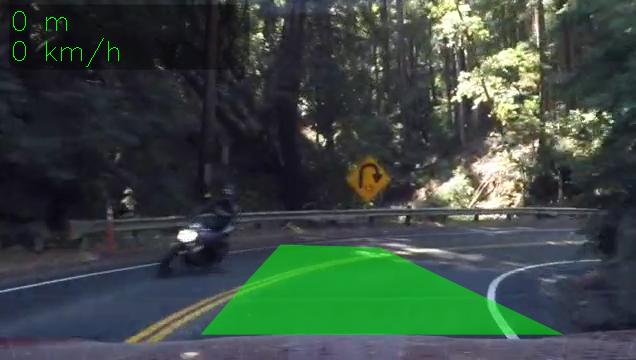
\includegraphics[max width=15cm,max height=15cm,keepaspectratio]{img_5_1}
	\caption{Detecție linii curbe}
\end{figure} 